\documentclass{article}
\usepackage{amsmath,amssymb, mathtools,dirtytalk}
\usepackage{graphicx} % Required for inserting images
\graphicspath{{Images/}}

\setlength{\oddsidemargin}{0in}
\setlength{\textwidth}{6.5in}
\setlength{\topmargin}{-.55in}
\setlength{\textheight}{9in}
\pagestyle{empty}


\title{Scientific Computation II HW2}
\author{Michael Nameika}
\date{February 2023}

\begin{document}

\maketitle

\section*{Section 5 Problems}
\textbf{3.} Let $E_N = \inf_p\|p(x) - e^x\|_{\infty}$, where $\|f\|_{\infty} = \sup_{x \in [-1,1]}|f(x)|$, denote the error in degree $N$ minimax polynomial approximation to $e^x$ on $[-1,1]$. (a) One candidate approximation $p(x)$ would be the Taylor series truncated at degree $N$. From this approximation, derive the bound $E_N < ((N + 2)/(N+1))/(N+1)!$ for $N \geq 0$. (b) In fact, the truncated Taylor series falls short of optimal by a factor of about $2^N$, for it is known (see equation (6.75) of [Mei67]) that as $N \to \infty$, $E_N \sim 2^{-N}/(N+1)!$. Modify Program 9 to produce a plot showing this asymptotic formula, the upper bound of (a), the error when $p(x)$ is obtained from interpolation in Chebyshev points, and the same for equispaced points, all as a function of $N$ for $N = 1, 2,3, \dots, 12$. Comment on the results.
\newline\newline
\begin{itemize}
    \item[(a)] Recall that 
    \[e^x = \sum_{k=0}^{\infty} \frac{x^k}{k!}\]
    Let $p(x)$ be the $N^{\text{th}}$ degree Taylor polynomial expansion of $e^x$. Then 
    \begin{align*}
        \|p(x) - e^x \|_{\infty} &= \sup_{x\in [-1,1]} \left| \sum_{k=N+1}^{\infty} \frac{x^k}{k!}\right| \\
        &= \sup_{x \in [-1,1]} \left| \frac{1}{(N+1)!} + \frac{1}{(N+2)!} + \hdots \right| \\
        &= \frac{1}{(N+1)!} + \frac{1}{(N+2)!} + \hdots \\
        &= \frac{1}{(N+1)!}\left( 1 + \frac{1}{N+2} + \frac{1}{(N+3)(N+2)} + \hdots \right) \\
        &<\frac{1}{(N+1)!}\left( \sum_{k=0}^{\infty} \frac{1}{(N+2)^k} \right) \\
        &= \frac{1}{(N+1)!}\left( \frac{1}{1 - \frac{1}{N+2}} \right) \\
        &= \frac{1}{(N+1)!}\left( \frac{N+2}{N+1} \right) \\
        &= \frac{\frac{N+2}{N+1}}{(N+1)!} \\
    \end{align*}
    So we have
    \[\|p(x) - e^x\|_{\infty} < ((N+2)/(N+1))/(N+1)!\]
    Which is what we sought to show.

    \item[(b)] Modifying program 9 to use the function $e^x$ and plotting the error from the interpolation on equispaced nodes and Chebyshev nodes, we find the following semilog plot:
    \begin{center}
        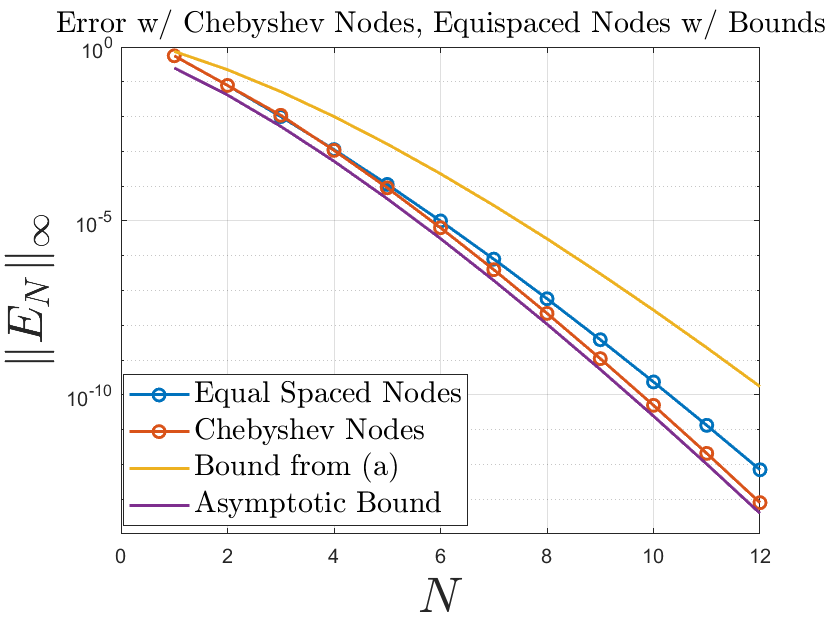
\includegraphics[scale = 0.6]{errorBounds}
    \end{center}
    Notice that the error from the Chebyshev nodes appears to follow closely to the asymptotic result as $N$ increases, as we would expect. Further notice how the error from the equispaced points appear to follow the trend of the bound we found in part (a).
\end{itemize}

\section*{Section 6 Problems}
\textbf{1.} If $x_0, x_1, \dots, x_N \in \mathbb{R}$ are distinct, then the \textit{cardinal function} $p_j(x)$ defined by 
\[p_j(x) = \frac{1}{a_j}\prod_{\substack{k=0\\k\neq j}}^N (x-x_k), \:\:\:\:\; a_j = \prod_{\substack{k=0\\ k\neq j}}^N (x_j - x_k)\]
is the unique polynomial interpolant of degree $N$ to the values 1 at $x_j$ and 0 at $x_k$, $k \neq j$. Take the logarithm and differentiate to obtain
\[p_j'(x) = p_j(x)\sum_{\substack{k=0\\ k\neq j}}^N (x - x_k)^{-1}\]
and from this derive the formula
\[D_{ij} = \frac{1}{a_j} \prod_{\substack{k=0\\ k\neq i,j}}^N(x_i - x_k) = \frac{a_i}{a_j(x_i - x_j)} \:\:\:\: (i \neq j)\]
and
\[D_{jj} = \sum_{\substack{k=0\\ k\neq j}}^N (x_j - x_k)^{-1}\]
\noindent\rule{12cm}{0.4pt}

Taking the logarithm of the equation for $p_j(x)$ above, we find
\begin{align*}
    \ln{(p_j(x))} &= \ln{\left(\frac{1}{a_j}\sum_{\substack{k=0\\ k\neq j}}^N (x -x_k)\right)}\\
    &= \ln{\left(\frac{1}{a_j}\right)} + \sum_{\substack{k=0\\ k\neq j}}^N \ln{(x - x_k)}
\end{align*}
Differentiating, we find 
\begin{align*}
    \frac{1}{p_j(x)}p'_j(x) &= \sum_{\substack{k = 0\\ k\neq j}}^N (x-x_k)^{-1}\\
    p'_j(x) &= p_j(x)\sum_{\substack{k=0\\k\neq j}}^N (x-x_k)^{-1}
\end{align*}
Plugging in $x_i$, $0 \leq i \leq N$, $i \neq j$, for $x$, we find
\begin{align*}
    p_j'(x_i) &= p_j(x_i)\sum_{\substack{k=0\\k\neq j}}^N(x_i - x_k)\\
    &= \frac{1}{a_j}\prod_{\substack{k = 0\\ k \neq j}}^N(x_i-x_k)\left(\sum_{\substack{k=0\\k\neq j}}^N(x_i - x_k)^{-1}\right)\\
    &= \frac{a_i}{a_j(x_i - x_j)}
\end{align*}
(since all terms go to zero except for the $k=i$ term)\newline
If $i = j$, then
\begin{align*}
    p_j'(x_j) &= \frac{1}{a_j}\prod_{\substack{k=0\\k\neq j}}^N(x_j - x_k) \left(\sum_{\substack{k=0\\k \neq j}}^N(x_j - x_k)^{-1}\right)\\
    &= \frac{a_j}{a_j}\sum_{\substack{k=0\\k\neq j}}^N(x_j - x_k)^{-1}\\
    &= \sum_{\substack{k=0 \\k\neq j}}^N(x_j - x_k)^{-1}\\
\end{align*}
Finally, we have 
\begin{align*}
    D_{ij} &= \frac{a_i}{a_j(x_i - x_j)} \:\:\:\:\:\: (i \neq j)\\
    D_{jj} &= \sum_{\substack{k= 0\\k \neq j}}^N(x_j - x_k)^{-1}
\end{align*}
Which is what we sought to show.
\newline\newline\newline
\textbf{8.} Let $D_N$ be the usual Chebyshev differentiation matrix. Show that the power $(D_N)^{N+1}$ is identically equal to zero. Now try it on the computer for $N=5$ and 20 and report the compupted 2-norms $\|(D_5)^6\|_2$ and $\|(D_{20})^{21}\|_2$. Discuss.
\newline\newline
Proof: Recall that the rows of the Chebyshev differentiation matrix are given by differentiating the $N$th degree interpolating polynomial $p(x)$ and inputting the Chebyshev nodes. Thus, since $p(x)$ is an $N$th degree polynomial,
\[\frac{d^{N+1}}{dx^{N+1}}p(x) = 0\]
That is, each element of the $(N+1)$th differentiation matrix is identically equal to zero.
\newline\newline
Using my chebDiffMat.m file, we find the following for $D_5$, $(D_5)^6$, and $\|(D_5)^6\|_2$:
\begin{center}
    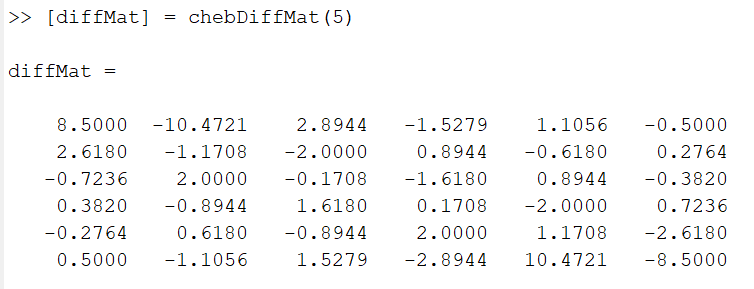
\includegraphics[scale = 0.75]{6_8_cheb5}
    \newline
    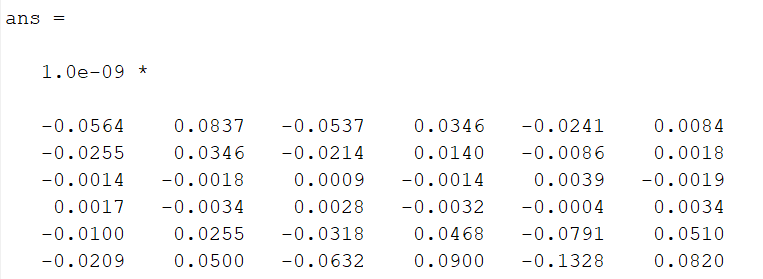
\includegraphics[scale = 0.65]{6_8_cheb5_nil}
    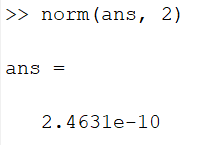
\includegraphics[scale = 0.7]{6_8_cheb5_svd}
\end{center}
So we can see that $(D_5)^6$ is essentially the zero matrix. However, for $D_{20}$, we find the following for $\|(D_{20})^{21}\|_2$:
\begin{center}
    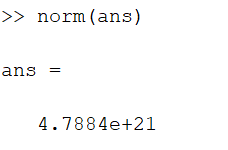
\includegraphics[scale = 0.9]{6_8_cheb20_sv}
\end{center}
This tells us that $(D_{20})^{21}$ is not even close to the zero matrix, when we expect it should be! This is likely due to machine round off error compounding with each successive power of $D_{20}$.

\section*{Section 7 Problems}
\textbf{1.} Modify Program 13 so that instead of polyval and polyfit, it uses the more stable formula of \textit{barycentric interpolation} [Hen82]:
\[p(x) = \sum_{j=0}^N\frac{a_j^{-1}u_j}{(x - x_j)}\bigg/\sum_{j=0}^N\frac{a_j^{-1}}{x-x_j}\]
where $\{a_j\}$ are defined by (6.7). Experiment with various interpolation problems (such as that of Exercise 5.1) and find evidence of the enhanced stability of this method.
\newline\newline
Implementing the barycentric interpolation formula (see the attached myProb13Script.m file), we find the following plots for the Runge function $f(x) = 1/(1 + 16x^2)$ and the solution to the differential equation $u_{xx} = e^{4x}$, $u(\pm 1) = 0$:
\begin{center}
    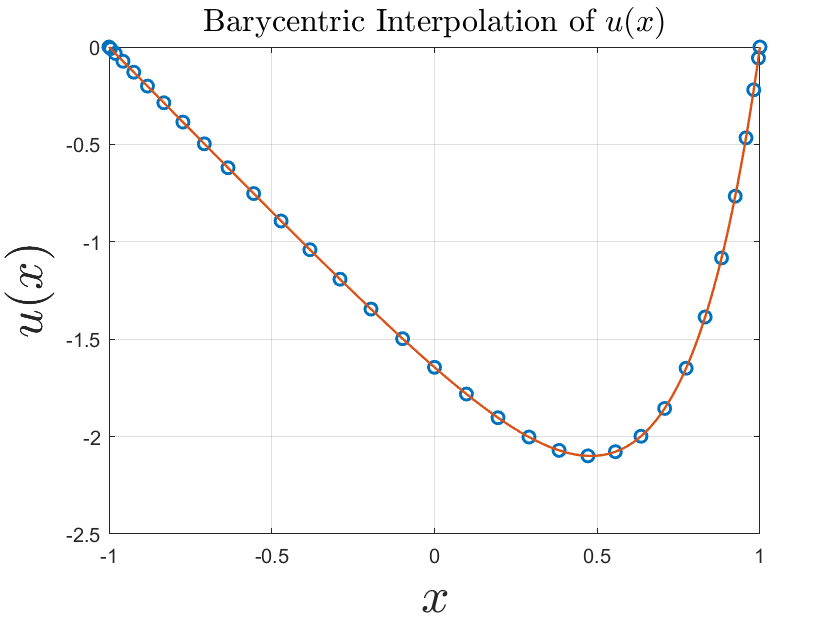
\includegraphics[scale = 0.35]{BarycentricInterpolation1}
    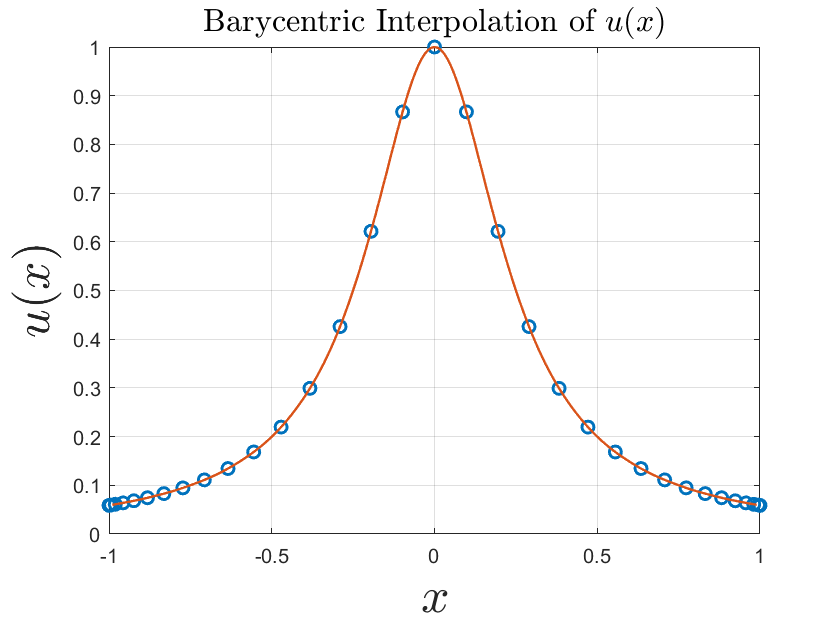
\includegraphics[scale = 0.35]{barycentricinterpolationRunge}
\end{center}
Increasing the number of interpolation points to $N = 64$, we find the following issue with the \say{normal} interpolation
\begin{center}
    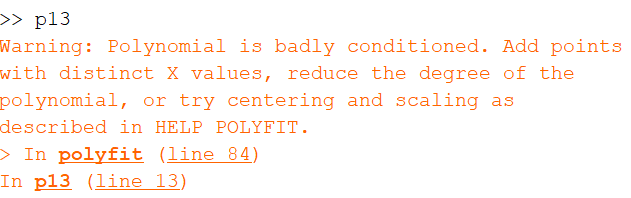
\includegraphics[scale = 0.9]{err}
\end{center}
Whereas the barycentric interpolation runs no problem:
\begin{center}
    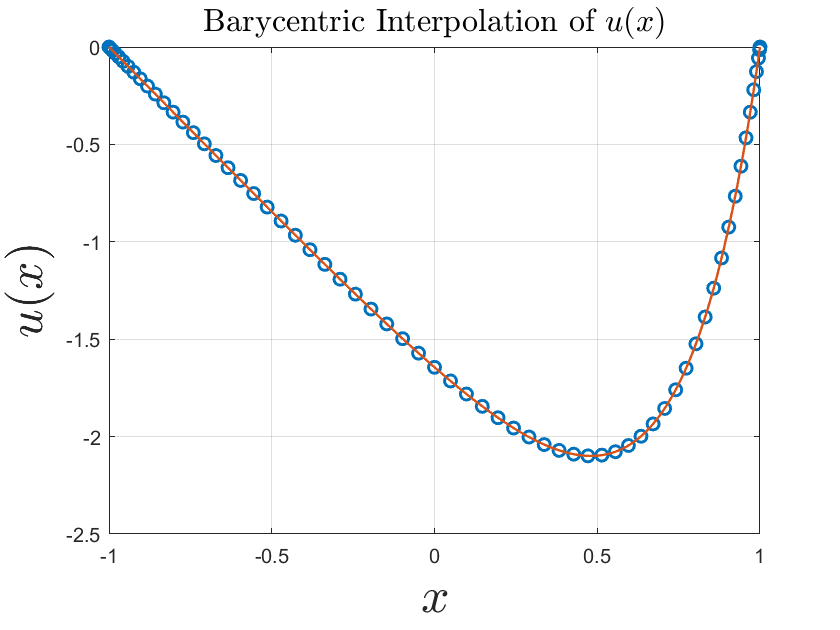
\includegraphics[scale = 0.4]{barycentric64}
\end{center}

\textbf{2.} Solve the boundary value problem $u_{xx} + 4u_x + e^xu = \sin(8x)$ numerically on $[-1,1]$ with boundary conditions $u(\pm 1) = 0$. To 10 digits of accuracy, what is $u(0)$?
\newline\newline
Implementing this ode in MATLAB using Chebyshev differentiation, we find the following solution plot:
\begin{center}
    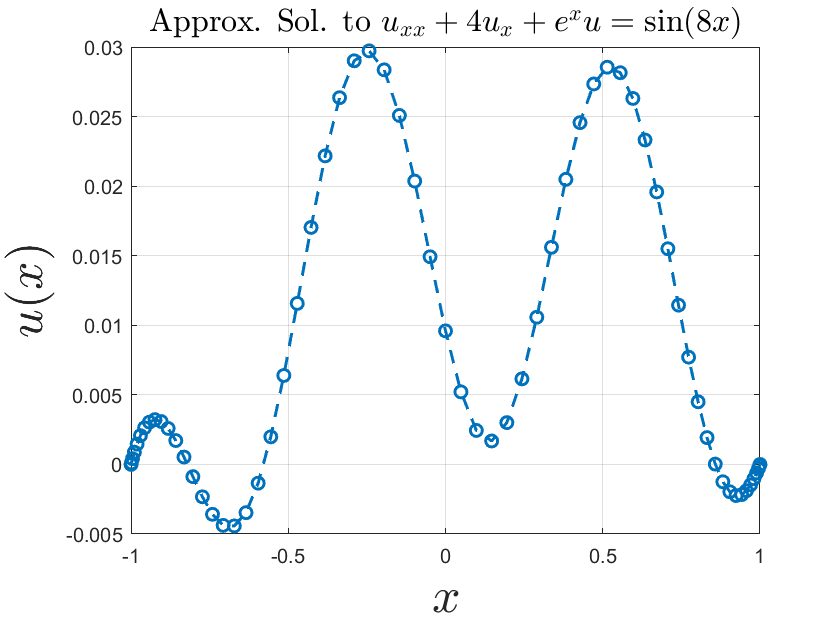
\includegraphics[scale = 0.6]{7_2_sol_plot}
\end{center}
And we find the following approximate value for $u(0)$:
\begin{center}
    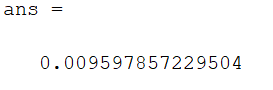
\includegraphics[scale = 1]{u(0)}
\end{center}
For this problem, we used $N = 64$. See the attached probScript.m for additional details.

\section*{Section 8 Problems}
\textbf{3.} Modify Program 12 (p. 57) to make use of chebfft instead of cheb. The results should be the same as in Output 12, except for rounding errors. Are the effects of rounding errors smaller or larger than before?
\newline\newline

Modifying Program 12 to use the chebfft file rather than cheb, we find the following plots:
\begin{center}
    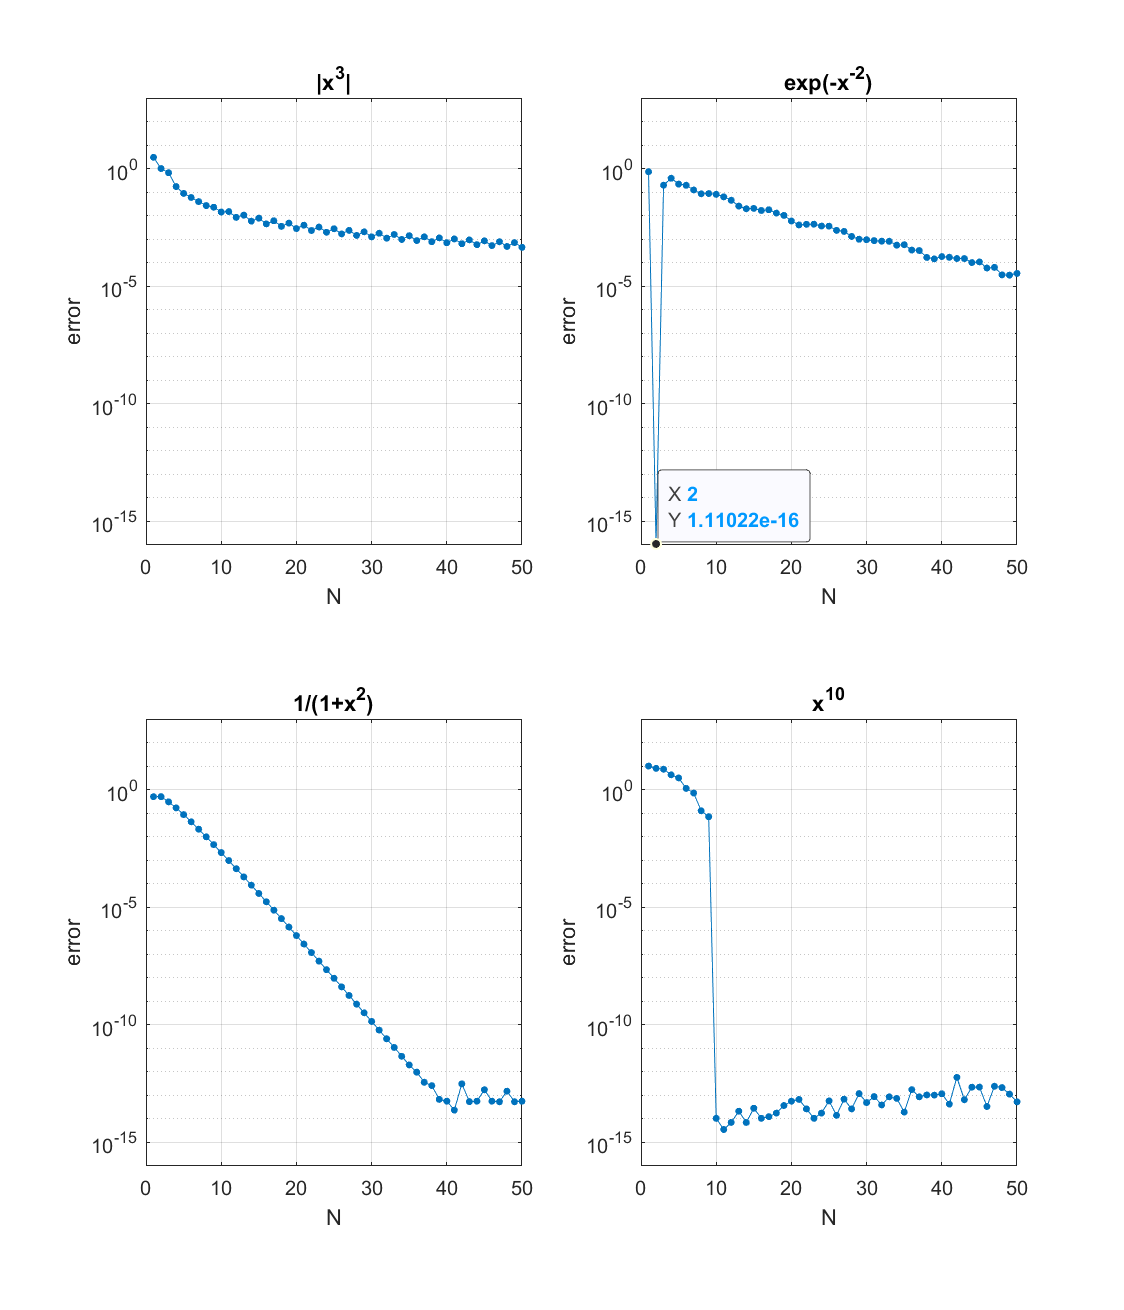
\includegraphics[scale = 0.25]{ChebyshevDiffMat}
    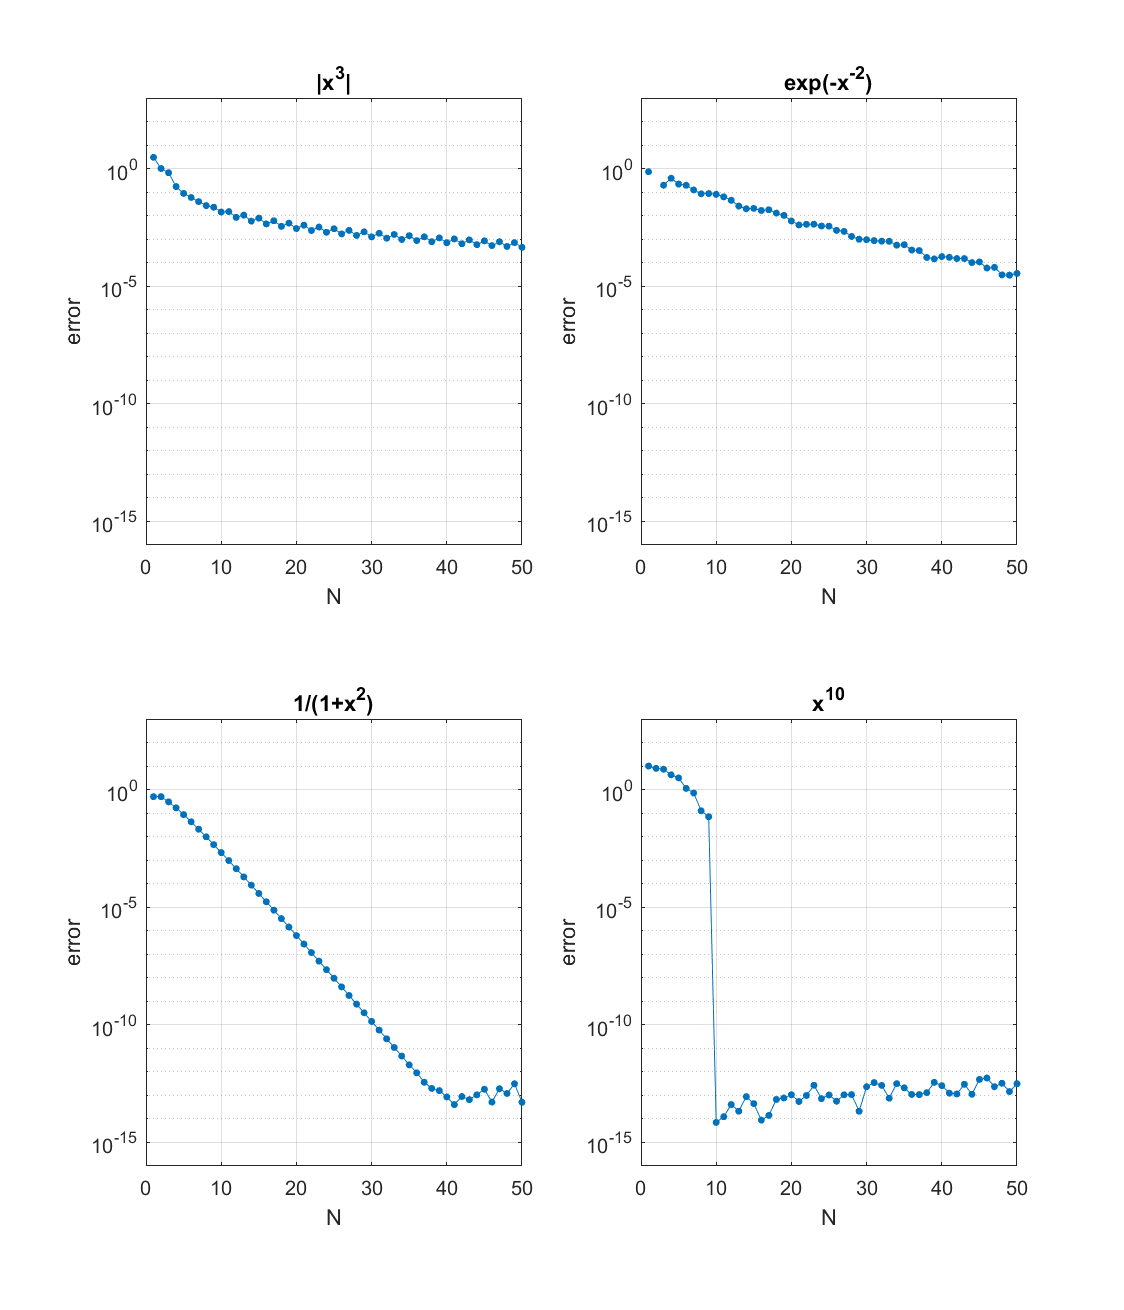
\includegraphics[scale = 0.25]{ChebFFT}
\end{center}
Above: Left figure shows Program 12 using cheb and the right figure shows Program 12 using chebfft. Notice the extreme similarities between the two plots. We can see that the rounding errors are approximately the same between the two figures, with the chebfft differentiation having smaller rounding errors and larger rounding errors when compared to the cheb differentiation matrix.
\newline\newline

\textbf{5.} Find a way to modify your program of Exercise 8.4, as in Exercise 3.8 but now for a second-order problem, to make use of matrix exponentials rather than time discretization. What effect does this have on the computation time?
\newline\newline
Starting with the two dimensional wave equation with $c = 1$,
\[\frac{\partial^2u}{\partial t^2} = \frac{\partial^2u}{\partial x^2} + \frac{\partial^2u}{\partial y^2}\]
and reducing to a system of first order equations in time, we have
\[\frac{d}{dt}\begin{bmatrix}
    u\\
    v
\end{bmatrix} = \begin{bmatrix}
    0 & I\\
    D & 0
\end{bmatrix}\begin{bmatrix}
    u\\
    v
\end{bmatrix}\]
Where $D$ is an $(N+1)^2$ by $(N+1)^2$ differentiation matrix, $0$ is the zero matrix with the same dimension, $I$ is the identity matrix of the same dimension, and $v = u_t$.
\newline
Let $\mathcal{L} = \begin{bmatrix}
    0 & I\\
    D & 0
\end{bmatrix}$ and multiply the above equation by $e^{\mathcal{L}t}$, we get
\[e^{\mathcal{L}t}\frac{d}{dt}\begin{bmatrix}
    u\\
    v
\end{bmatrix} - \mathcal{L}e^{\mathcal{L}t}\begin{bmatrix}
    u\\
    v
\end{bmatrix} = 0\]
which becomes
\[\frac{d}{dt}\left(e^{\mathcal{L}t}\begin{bmatrix}
    u\\
    v
\end{bmatrix}\right) = 0\]
which gives us
\[e^{\mathcal{L}t}\begin{bmatrix}
    u\\
    v
\end{bmatrix} = C\]
and for $t=0$, we find $C = \begin{bmatrix}
    u(x,y,0)\\
    v(x,y,0)
\end{bmatrix}$
Then the general solution takes the following form:
\[\begin{bmatrix}
    u\\
    v
\end{bmatrix} = e^{-\mathcal{L}t}\begin{bmatrix}
    u\\
    v
\end{bmatrix}\]
Implementing this into MATLAB, we find the following plot for $N = 64$:
\begin{center}
    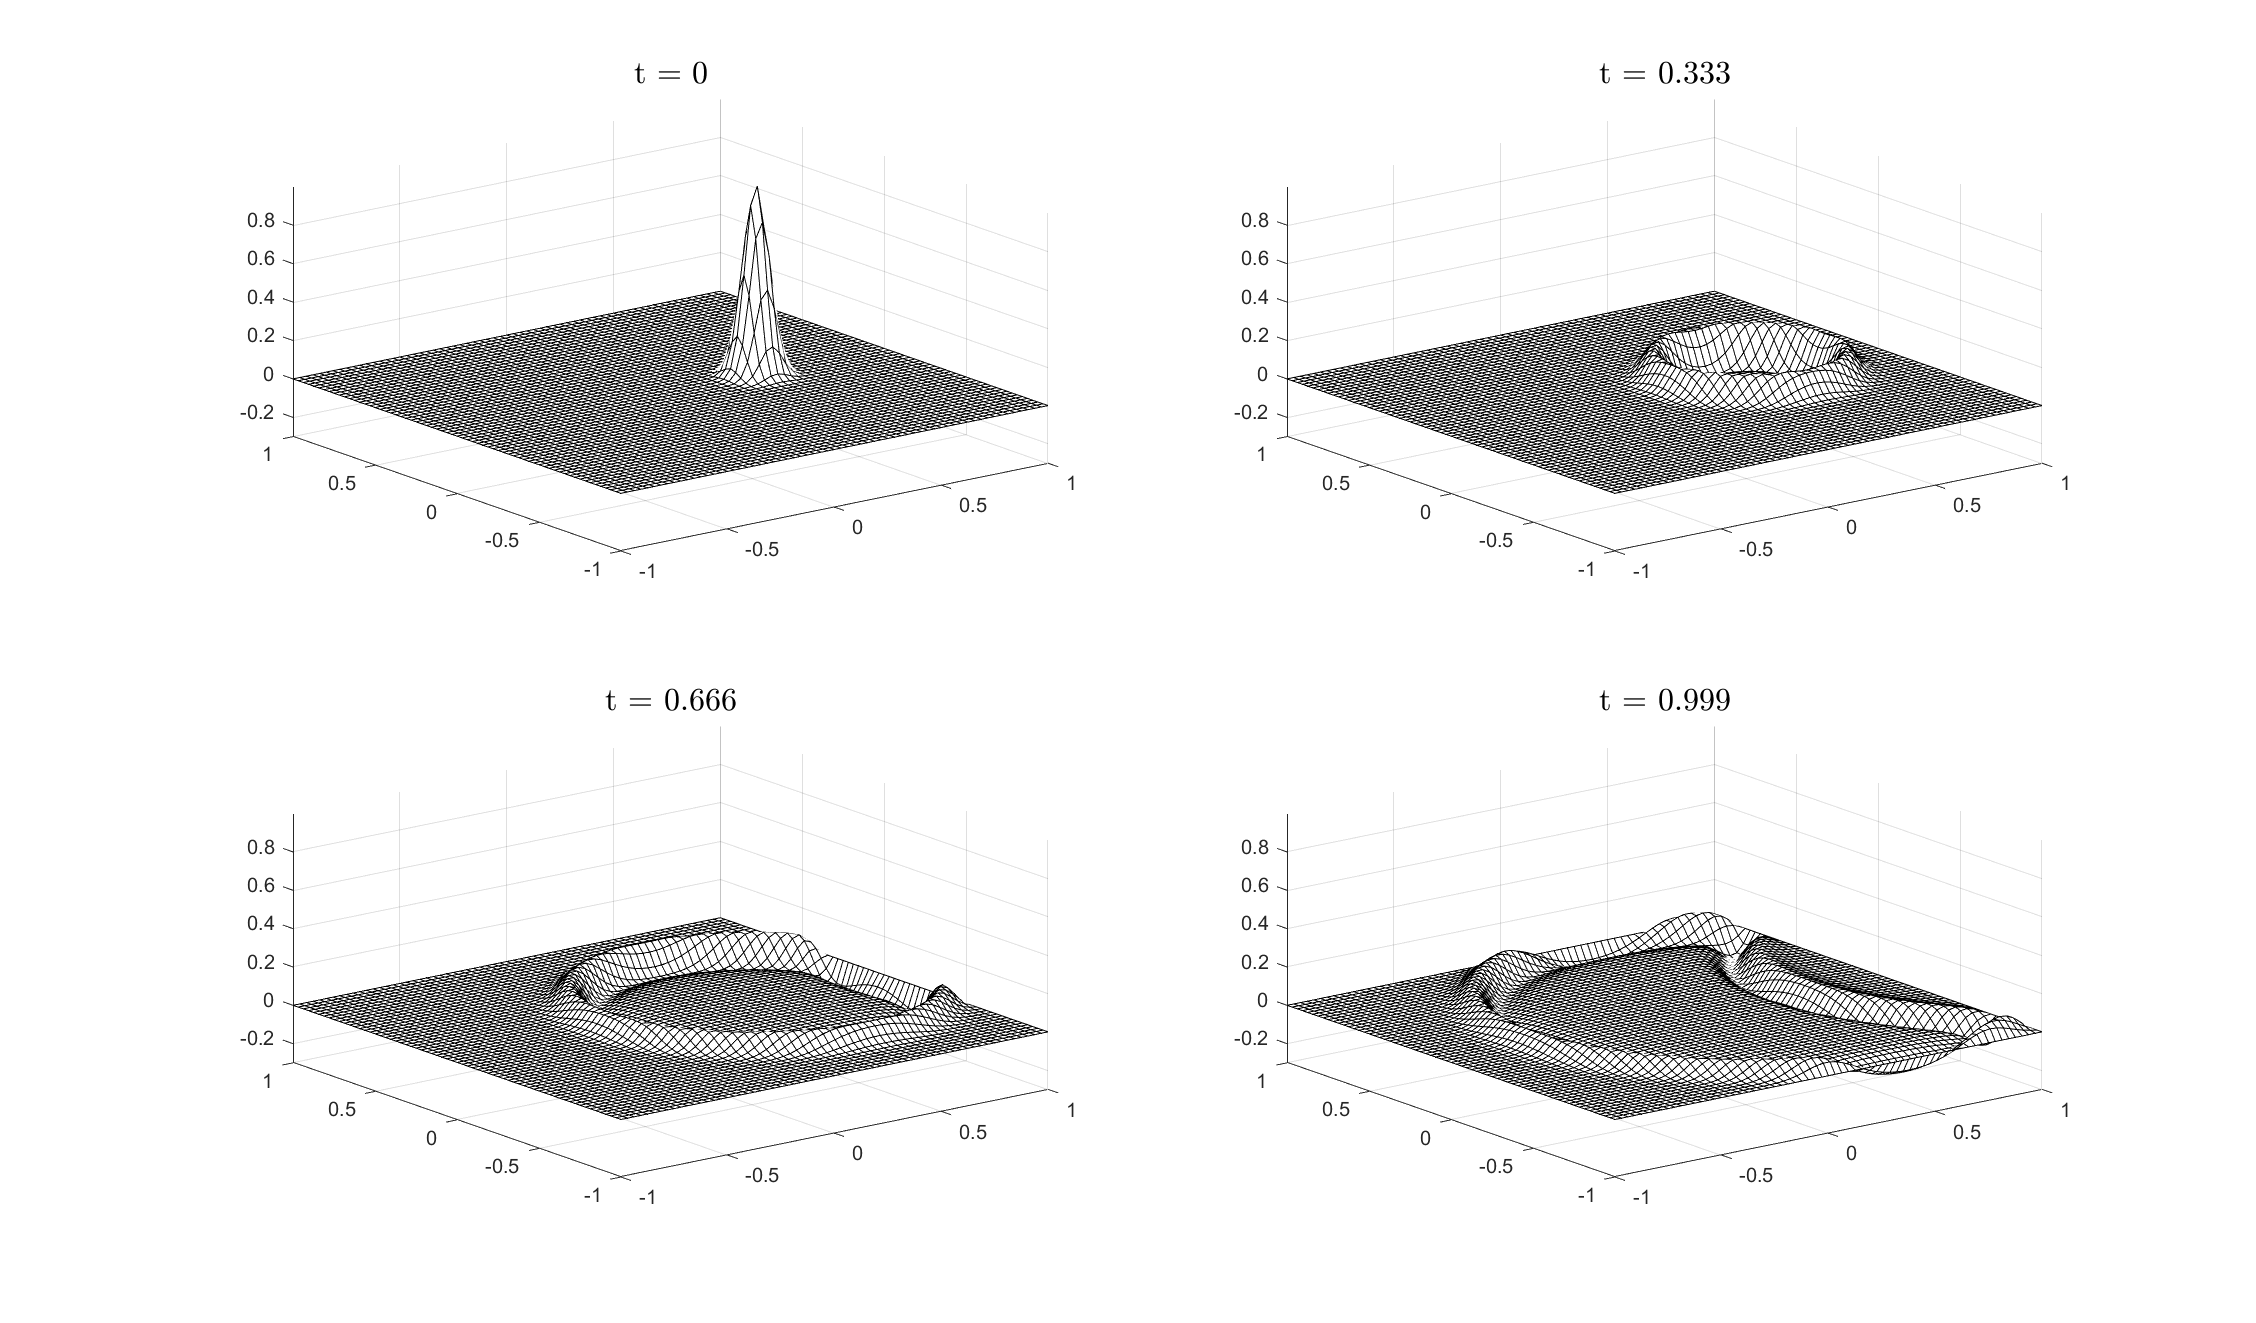
\includegraphics[scale = 0.25]{2DwaveEqwMatrixExponential}
\end{center}
Running it for $N = 64$ took nearly seven minutes, so this had a massive impact on the computation time!


\end{document}
